\documentclass[11pt]{article}
\renewcommand{\baselinestretch}{1.0}

\usepackage{amsfonts}
\usepackage{hyperref}
\usepackage{color}
\usepackage{graphicx}
\usepackage{fullpage}
\usepackage{booktabs}
\usepackage{pdfpages}
\usepackage{amsmath}
\usepackage{amssymb}
\pagestyle{empty}
\renewcommand{\baselinestretch}{1.0}
\newcommand{\ffrac}[2]{\ensuremath{\frac{\displaystyle #1}{\displaystyle #2}}}

\title{Statistics Project 1 : \\ Statistics - Math 2606}
\author{Kevin Chen, Will Gantt, Nick Barnes}
\date{}
\begin{document}
\maketitle
\section{Experiment}

The assignment was to estimate the height of Searles. Although it would have been ideal to estimate the height to the top of the spire, we did not do this. Instead, we measured to the point at the top of the front facade above the door. This approach has the advantage of not requiring that one estimate the horizontal distance from the spire to the front facade, which would introduce more error.

Let the $x$-axis be the imaginary line passing through the door, parallel to the walkway that passes in front of the building, and let the $y$-axis be the line passing through the door, perpendicular to the walkway. For all measurements, we maintained a constant distance from the $x$-axis. We chose this value to be the distance from the door to a point directly in front of it, at the far edge of the walkway, where the pavement meets the grass. Call this value $a$. To vary the distance from the door to the mirror, we marked out 10 positions at 2m-intervals along the line defined by $a$ that is parallel to the $x$-axis. Call that distance to the point directly in front of the door $b$. Then our direct distance to the base of the building directly below the top of the front facade above the door is $\sqrt{a^2+b^2}$. This is a simple application of the Pythagorean theorem, as our distance from the point directly in front of the door, and our distance from the point on the line parallel to the x-axis are perpendicular. 

Note that the error obtained in measuring the distance from the point directly in front of the door, and the error in measuring distance from the mirror to that point do \textbf{not} add up linearly. That is, call them $\epsilon_1$ and $\epsilon_2$, and the distance from the point perpendicular to the building $a$, the distance from the point perpendicu [FOR KEVIN TO FINISH]

Will acted as the observer for all trials. His height ($h_1$) was measured 10 times with a tape measure, once for each trial. The distances $a$ and $b$ (together determining $d_2$), as well as the distance from Will to the mirror ($d_1$), were determined by extending a length of string the desired distance, marking the string, and then measuring the string with the tape measure. Measurements for $b$ and $d_1$ were also taken 10 times, but we used the same value of $a$ throughout.\footnote{We recognize that this is a mistake and that we should have measured $a$ 10 times as well.} All measurements are shown in Fig. 1. The value obtained for $d_2$ in measurement 1 shown in the figure was the value we used for $a$.

\section{Results}
From our 10 trials, we inferred the value of $h_2$ to be about 16.64m. Our mean values for $h_1$, $d_1$, and $d_2$ can also be found in Fig. 1. Our estimates for the standard deviation of the measurements, up to an order of magnitude, are as follows:
\begin{align*}
\sigma_{h_1} &= 1\text{cm} \\
\sigma_{d_1} &= 1\text{dm} \\
\sigma_{d_2} &= 1\text{m}
\end{align*}

To determine the impact of the error on the inferred value of $h_2$, we need to understand the change in the height of Searles with regard to a change in the distance from the mirror to the base of Searles, the mirror to Will, and the height of Will. We simply take the partial derivatives with respect to each quantity to understand how the height of Searles depends on these measurements. \\
\begin{align*}
    \frac{\partial}{\partial H_w} &= \frac{D_s}{D_w} \\
	\frac{\partial}{\partial H_s} &= \frac{H_w}{D_w} \\
	\frac{\partial}{\partial D_s} &= -D_w^{-2}D_sH_w = -\frac{D_sH_w}{D_w^2} \\
\end{align*}
Now we can calculate the values of these derivatives using an average value for $D_s, H_w, D_w$ and multiply these derivatives with their estimated standard deviations, respectively, and the largest value should be the error that has the greatest impact on our calculated height [FOR KEVIN TO FINISH].

The plots below show, respectively, $d_1$, $d_2$, and $h_1$ graphed against inferred values for $h_2$. The vertical line in each plot represents the mean value of the parameter on the $x$-axis ($d_1$, $d_2$, or $h_1$), and the horizontal line represents the mean height of Searles (16.64m). These lines allow us to visualize the deviation of each measurement from the mean value of the corresponding parameter.

The curious thing is that the graphs show no clear relationship between any of $d_1$, $d_2$, and $h_1$ on the one hand, and $h_2$ on the other. For all of our calculations, we posited a model of additive error. Moreover, we showed that, based on that model, the error in $d_1$ should correlate most strongly with the error in $h_2$. (To frame it another way: a change in $d_1$ should produce a greater change in $h_2$ than either $h_1$ or $d_2$ would produce.) And yet, the graphs provide no evidence for such a conclusion. There seem to be two inferences we could draw from these results:
\begin{enumerate}
\item Our data collection was sufficiently imprecise to obscure a relationship between the measurements that does in fact exist.
\item The model of additive error that we posited is not an accurate representation of reality.
\end{enumerate}
We believe that although there were problems with our data collection, it is likely the case that the model of additive error is not a good one for the purposes of this experiment.
\begin{figure}
\label{measurements}
\centering
\begin{tabular}{ccccc}
\toprule
Measurement \# & $h_1$ & $d_1$ & $d_2$ & $h_2$ \\
\midrule
1 & 1.78 & 1.12 & 10.86 & 17.26 \\
2 & 1.77 & 1.2 & 11.04 & 16.28 \\
3 & 1.76 & 1.25 & 11.57 & 16.29 \\
4 & 1.77 & 1.41 & 12.41 & 15.58 \\
5 & 1.77 & 1.46 & 13.49 & 16.35 \\
6 & 1.77 & 1.66 & 14.76 & 15.74 \\
7 & 1.76 & 1.69 & 16.18 & 16.85 \\
8 & 1.77 & 1.84 & 17.72 & 17.05 \\
9 & 1.78 & 1.87 & 19.34 & 18.41 \\
10 & 1.77 & 2.25 & 21.02 & 16.54 \\
\midrule
mean & 1.77 & 1.575 & 14.839 & 16.635 \\
\bottomrule
\end{tabular}
\caption{Measurements for iris height ($h_1$), the distance from the mirror to Will ($d_1$), the distance from Searles to the mirror ($d_2$), and the resultant estimate of the height of Searles ($h_2$). All units are in meters.}
\end{figure}

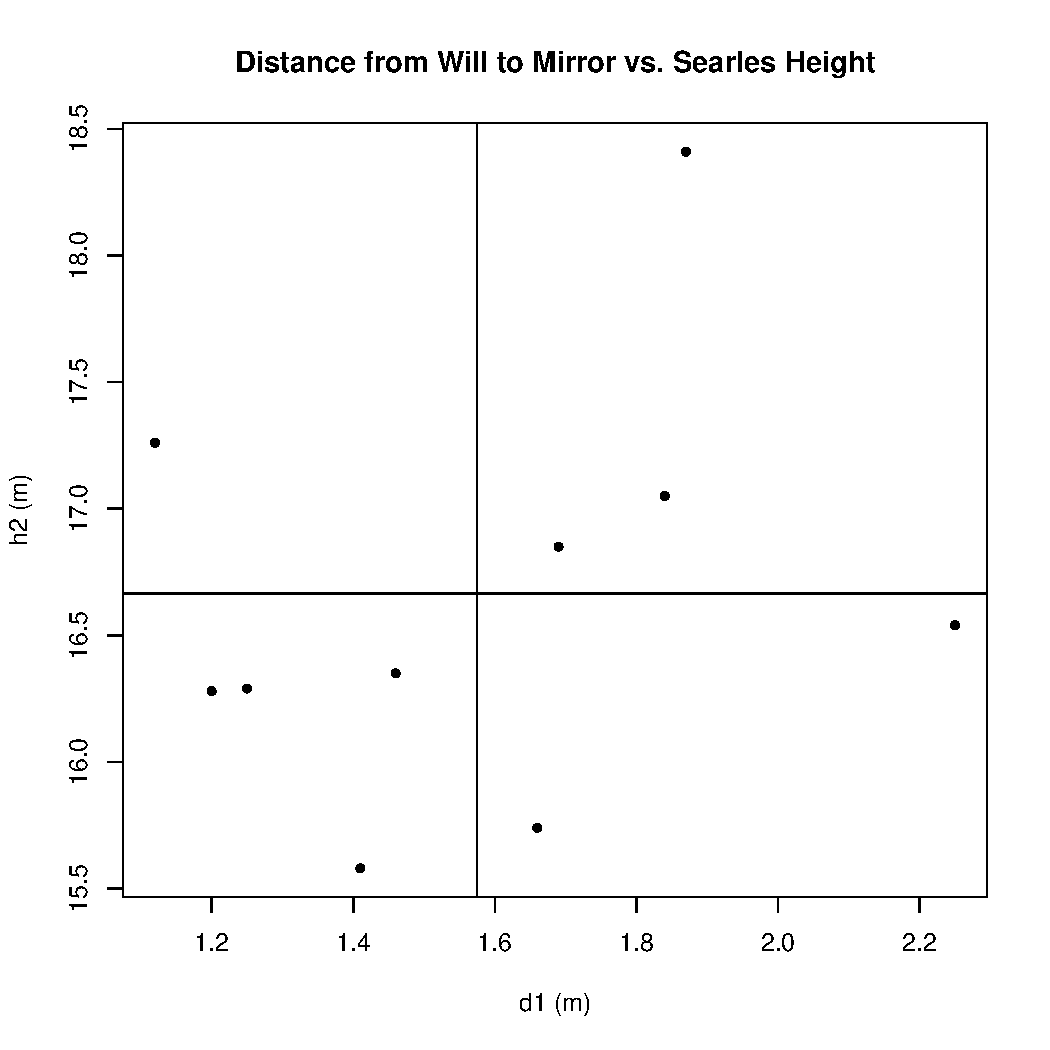
\includepdf[scale=0.8]{d1_h2.pdf}
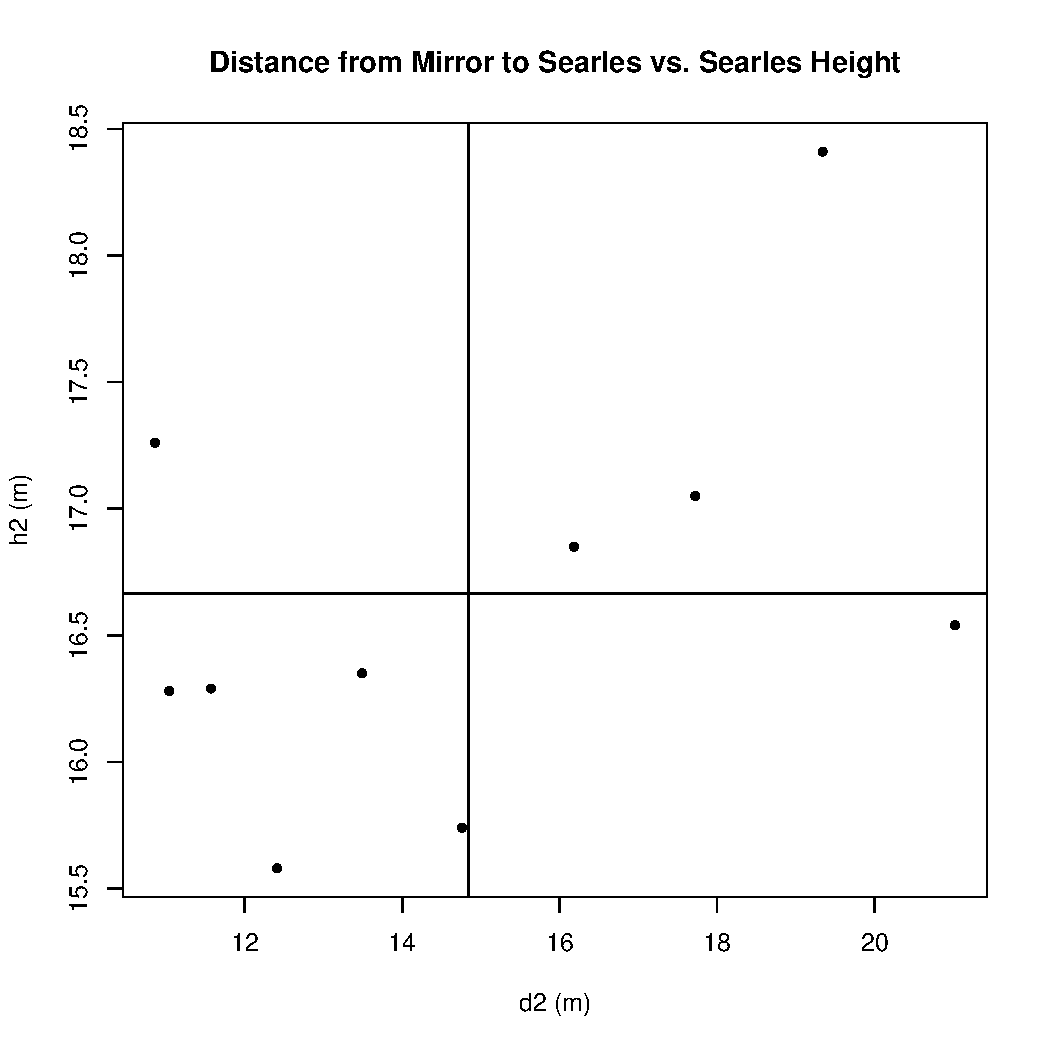
\includepdf[scale=0.8]{d2_h2.pdf}
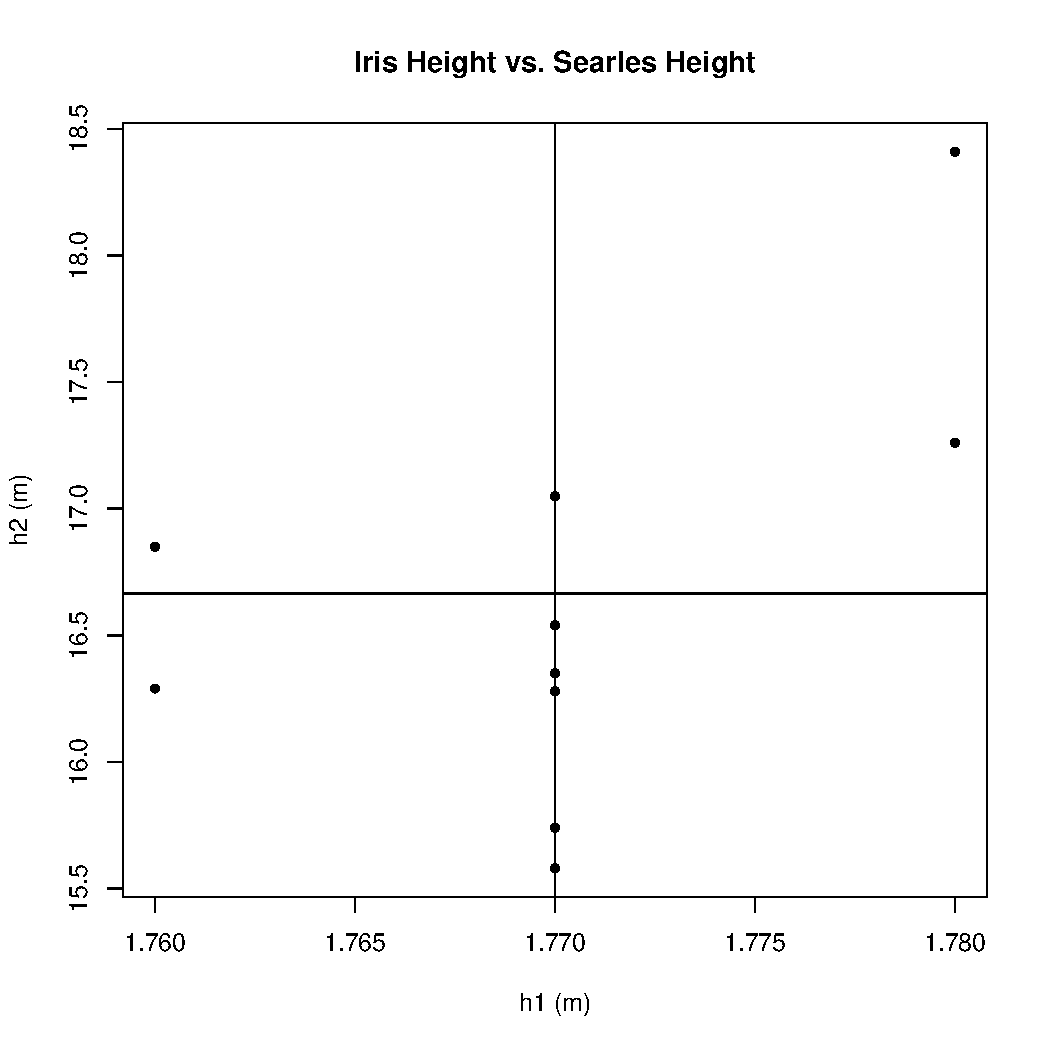
\includepdf[scale=0.8]{h1_h2.pdf}

\end{document}